\section{Introduction}
\label{introduction}

% 大背景
% GNN-based predictors have become an important class of learning-based surrogates for AI-assisted EDA, where many prediction tasks are defined over graph-structured design artifacts. They have been widely explored for resource estimation, timing prediction, congestion analysis, and design-space exploration, providing fast approximations to expensive EDA tools in modern design flows.

% % 观察到的现象，和现象解释
% Despite this promise, deploying GNN predictors across EDA tasks is not a plug-and-play process. Strong EDA GNN predictors are often not determined by the choice of a generic backbone alone. Their effectiveness often depends on whether the graph-learning problem is formulated to reflect the reasoning structure of the target EDA analysis. Timing prediction provides a representative example: an effective predictor must expose timing-relevant objects, propagate delay-related information along circuit dependencies, and use meaningful intermediate timing quantities to guide learning beyond the final label.
% {\color{blue}[Fig1]}

  
% This difficulty is intrinsic to EDA prediction. Unlike ordinary graph labels, EDA labels are tool-induced properties computed over realized design states, for example after synthesis, implementation, or scheduling. Rather than directly annotating isolated graph nodes or edges, these labels summarize task-specific analyses over hidden design states and constraints. When a predictor is given only a generic graph and the final label, these task semantics remain implicit, forcing the model to recover them statistically from data. This makes EDA prediction an under-specified and data-inefficient inverse problem, where the model may exploit superficial label correlations instead of learning the analysis structure that gives rise to the target property. The core issue is thus not merely whether the GNN backbone is expressive enough, but whether the learning formulation exposes the task objects, dependencies, and intermediate quantities needed to make the target EDA analysis learnable.

% % 现象蕴含出的方法论
% This observation shifts the design target from choosing a better GNN backbone to formulating a better EDA graph-learning problem. We call this process \textit{semantic co-design}: graph representation, GNN computation, and learning signal are designed as mutually consistent realizations of the same task-level hypothesis about how an EDA property is produced. 
% % In this view, the key question is not only which neural primitive to use, but also what design objects should be exposed, how task-relevant information should propagate, and which intermediate quantities should shape the learned representationl
% {\color{blue}[Fig2]}

% \begin{figure}[tb!]
%   \centering

%   \subfloat[]{%
%     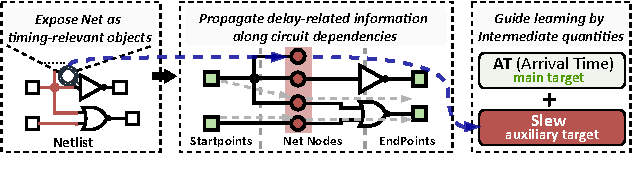
\includegraphics[width=1\linewidth]{figs/Q-1.pdf}
%     \label{fig:problem-1}
%   }\\[-0.1em]

%   \subfloat[]{%
%     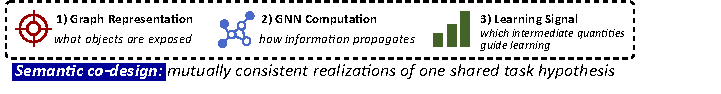
\includegraphics[width=1\linewidth]{figs/Q-2.pdf}
%     \label{fig:problem-2}
%   }\\[-0.8em]   % 重点：减小 b 和 c/d 之间的距离

%   \subfloat[]{%
%     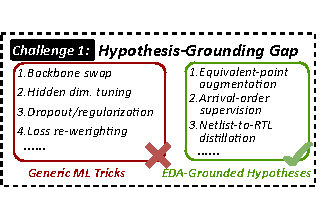
\includegraphics[width=0.49\linewidth]{figs/Q-3.pdf}
%     \label{fig:problem-3}
%   }
%   \hfill
%   \subfloat[]{%
%     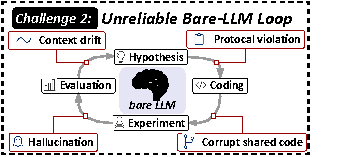
\includegraphics[width=0.48\linewidth]{figs/Q-4.pdf}
%     \label{fig:problem-4}
%   }

%   \caption{\textbf{TODO}}
%   \label{fig:problem}
% \end{figure}



% % 挑战部分
% Realizing semantic co-design requires searching beyond a fixed set of neural primitives. Since task-level modeling hypotheses are often easier to express in language than to enumerate as NAS operators, LLM agents offer a promising search mechanism: they can reason about the EDA task, propose meaningful hypotheses, and translate them into feature engineering, model or training improvement.

% However, two challenges limit their direct use. First, a \textit{hypothesis-grounding gap} arises because general-purpose agents tend to generate generic ML tricks, such as backbone replacement or hyperparameter tuning, rather than EDA-grounded hypotheses derived from design objects, tool semantics, structural dependencies, or intermediate analysis quantities. Second, an \textit{unreliable bare-LLM loop} makes long-horizon auto-research difficult: as the agent repeatedly performs hypothesis formulation, coding, experimentation, and evaluation, lengthy EDA tool reports and accumulating experimental states can cause context drift, hallucination, protocol violations, and unintended edits to shared code. Consequently, even runnable candidates may lack clear domain rationale, reliable comparison, and attributable evidence.
% {\color{red}[E5: hypothesis-grounding and bare-LLM reliability study.]}
% {\color{blue}[Fig3\&4]}

% % 方法 TODO
% To address these challenges, we propose \textbf{SCOPE}, a protocol-grounded agentic framework for EDA-native GNN design. SCOPE uses LLM agents to explore semantic co-design hypotheses beyond fixed NAS primitives. To preserve \textit{hypothesis grounding}, SCOPE organizes each candidate around three semantic levels---representation, computation, and learning signal---and requires the candidate to correspond to an explicit EDA modeling rationale. To preserve \textit{evidence attribution}, SCOPE evaluates each candidate through a scoped task interface and records it as a design trace that binds the hypothesis, implementation scope, training configuration, validation result, and parent-child relation. This allows SCOPE to keep the search space open enough for task-level modeling hypotheses, while making each discovered improvement comparable, replayable, and attributable.

% % Evaluation
% We evaluate SCOPE on representative AI EDA prediction tasks, including HLS resource prediction, netlist-level timing prediction, and RTL-to-netlist timing prediction. The evaluation examines whether SCOPE discovers EDA-native designs beyond conventional GNN-NAS spaces, whether its protocol improves attribution and reproducibility over naive LLM exploration, and whether the discovered predictors improve accuracy over human baselines and automated search baselines. {\color{red}[E6: final benchmark results to be inserted.]}

% The contributions are summarized as follows:
% \begin{itemize}
% \item \textbf{Observation.} We characterize effective EDA GNN design as \textit{semantic co-design}, where representation, computation, and learning signal are jointly aligned with the reasoning structure of the target EDA analysis. We support this characterization through literature taxonomy and controlled pre-experiments.

% \item \textbf{Method.} We introduce \textbf{SCOPE}, a protocol-grounded agentic framework that uses LLM agents to search EDA-native design hypotheses, while enforcing hypothesis grounding through semantic-level organization and evidence attribution through scoped interfaces and design traces.

% \item \textbf{Evaluation.} We evaluate SCOPE across representative EDA prediction tasks and compare it with human baselines, conventional GNN-NAS, and naive LLM-based exploration. {\color{red}[Experimental results to be inserted.]}

% \end{itemize}


\IEEEPARstart{G}{NN-based} predictors have become an important class of learning-based surrogates for AI-assisted electronic design automation (EDA), where many prediction tasks are defined over graph-structured design artifacts. They have been widely explored for resource estimation, timing prediction, congestion analysis, and design-space exploration, providing fast approximations to expensive EDA tools in modern design flows.
However, developing an effective GNN predictor for an EDA task is rarely a matter of selecting a stronger neural backbone alone. EDA prediction targets are produced by structured analysis procedures---such as synthesis, scheduling, static timing analysis, or physical implementation---and an effective learning formulation often needs to reflect the task-specific semantics underlying these procedures. In practice, many successful EDA GNNs therefore rely on manually designed choices about what design information should be exposed to the model, how task-relevant information should be propagated, and what intermediate semantics should guide learning. We refer to the coordinated design of these choices as \textit{semantic co-design}.

The automation of GNN design has evolved through two existing paradigms, yet both remain insufficient for EDA-native model research. \textbf{First, conventional GNN-NAS and AutoML} automate model selection within expert-defined search spaces, such as neural operators, aggregation functions, depth, normalization, and training hyperparameters. Their automation is therefore limited to choices that have already been enumerated. \textbf{Second, recent LLM-based research agents} remove this restriction by directly proposing and implementing open-ended code modifications, substantially expanding the space of possible designs. However, unrestricted exploration alone is not enough: as the search space becomes more open, useful research increasingly depends on \emph{narrowing} exploration toward hypotheses that are meaningful for the target domain. Motivated by this limitation, we propose a third paradigm for EDA GNN automation: \textbf{hypothesis-driven auto-research}, where the fundamental unit of exploration is neither a predefined architecture choice nor an arbitrary code patch, but an explicit EDA modeling hypothesis. The key is to retain the open-ended generation capability of LLM agents while progressively narrowing it into grounded and testable research directions.

Realizing hypothesis-driven AutoResearch introduces two challenges. \textbf{(1) Hypothesis-grounding gap:} open-ended agents often fall back to generic ML modifications, such as backbone replacement, hidden-dimension tuning, regularization, or loss reweighting, rather than hypotheses derived from EDA-specific objects, dependencies, and analysis semantics. \textbf{(2) Unreliable long-horizon execution:} even with a meaningful initial hypothesis, repeated hypothesis formulation, coding, experimentation, and evaluation can lead to context drift, uncontrolled code changes, protocol violations, and ambiguous attribution of performance improvements.

To address the first challenge, we use \textit{semantic co-design} to narrow open-ended hypothesis generation into three EDA-grounded levels: \textbf{representation}, which determines what task-relevant objects and dependencies are exposed; \textbf{computation}, which determines how task-relevant information propagates; and \textbf{learning signal}, which determines what intermediate EDA semantics guide learning. These levels do not enumerate concrete model candidates. Instead, they define where meaningful hypotheses should be sought, allowing the agent to generate previously unspecified designs while remaining grounded in the reasoning structure of the target EDA analysis.

To address the second challenge, we organize agent execution as a \textit{hypothesis tree}. Each node represents a hypothesis-backed research state, and each edge represents a controlled refinement of its parent. Rather than evolving a single long and entangled research trajectory, the agent can explicitly branch from promising states, compare alternative refinements, revisit earlier hypotheses, and prune ineffective directions. A scoped experimental protocol further binds each hypothesis to its implementation scope, training configuration, evaluation result, and lineage, making the resulting exploration replayable, comparable, and attributable.

Based on these mechanisms, we present \textbf{\sysname}, a hypothesis-driven AutoResearch harness for EDA-native GNN exploration. \sysname combines semantic narrowing with hypothesis-tree execution: semantic co-design determines \emph{what kinds of hypotheses are meaningful to explore}, while the hypothesis tree and scoped protocol determine \emph{how those hypotheses are reliably executed and refined}. Together, they preserve the flexibility of LLM-based exploration without reducing automated research to either a fixed NAS space or unconstrained trial-and-error.

% Evaluation
We evaluate \sysname on representative AI-for-EDA prediction tasks, including HLS resource prediction, netlist-level timing prediction, and RTL-to-netlist timing prediction. Our evaluation examines whether \sysname discovers EDA-native GNN designs beyond conventional GNN-NAS spaces, whether semantic grounding and hypothesis-tree execution improve research reliability over naive LLM exploration, and whether the discovered predictors outperform human-designed and automated-search baselines. {\color{red}[E6: final benchmark results to be inserted.]}

The contributions are summarized as follows:
\begin{itemize}
\item \textbf{Hypothesis-driven AutoResearch.} We introduce a new automation paradigm for EDA-native GNN research that moves beyond predefined architecture search and unconstrained LLM code exploration. The key principle is to preserve open-ended generation while narrowing it toward explicit, testable EDA modeling hypotheses.

```
\item \textbf{Semantic hypothesis grounding.} We use representation, computation, and learning signal as three semantic levels for narrowing open-ended exploration toward EDA-grounded hypotheses, without requiring experts to enumerate concrete candidate designs in advance.

\item \textbf{Hypothesis-tree execution.} We organize long-horizon agent exploration as a hypothesis tree with scoped experimental protocols, enabling controlled refinement, branching, replay, comparison, and evidence attribution across research trajectories.

\item \textbf{Evaluation.} We evaluate \sysname across representative EDA prediction tasks against human-designed baselines, conventional GNN-NAS, and naive LLM-based exploration. {\color{red}[Experimental results to be inserted.]}
```

\end{itemize}



